\begin{tabularx}{\linewidth}{|p{2.5cm}|X|X|X|X|}
\hline
\textbf{Item} 
& \textbf{$f(x)=(x+3)^2$} 
& \textbf{$f(x)=x(x+3)^2$} 
& \textbf{$f(x)=x^2(x+3)^2$} 
& \textbf{$f(x)=\dfrac{1}{x-2}$} \\
\hline

Graph &
\vspace{0pt}
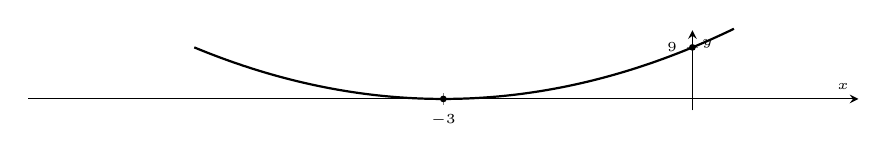
\begin{tikzpicture}[baseline=(current bounding box.north)]
\begin{axis}[
    width=\linewidth,
    height=2.6cm,
    axis lines=middle,
    xmin=-8, xmax=2,
    ymin=-2, ymax=12,
    xtick={-3},
    ytick={9},
    xticklabel style={font=\tiny},
    yticklabel style={font=\tiny},
    label style={font=\tiny},
    enlargelimits=false,
    samples=100,
    domain=-6:0.5,
    clip=false,
    xlabel={$x$},
    ylabel={$y$},
]
\addplot[thick] {(x+3)^2};
\addplot[only marks, mark=*, mark size=1pt] coordinates {(-3,0) (0,9)};
\end{axis}
\end{tikzpicture}
&
\vspace{0pt}
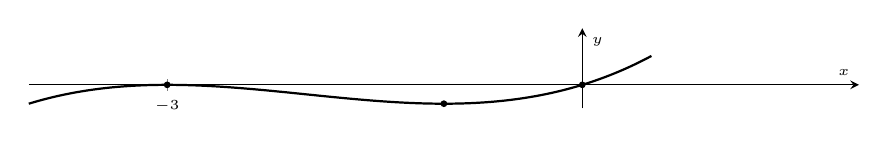
\begin{tikzpicture}[baseline=(current bounding box.north)]
\begin{axis}[
    width=\linewidth,
    height=2.6cm,
    axis lines=middle,
    xmin=-4, xmax=2,
    ymin=-5, ymax=12,
    xtick={-3,0},
    ytick=\empty,
    xticklabel style={font=\tiny},
    yticklabel style={font=\tiny},
    label style={font=\tiny},
    enlargelimits=false,
    samples=200,
    domain=-4:0.5,
    clip=false,
    xlabel={$x$},
    ylabel={$y$},
]
\addplot[thick] {x*(x+3)^2};
\addplot[only marks, mark=*, mark size=1pt] coordinates {(-3,0) (0,0) (-1,-4)};
\end{axis}
\end{tikzpicture}
&
\vspace{0pt}
\begin{tikzpicture}[baseline=(current bounding box.north)]
\begin{axis}[
    width=\linewidth,
    height=2.6cm,
    axis lines=middle,
    xmin=-8, xmax=2,
    ymin=-1, ymax=12,
    xtick={-3,0},
    ytick=\empty,
    xticklabel style={font=\tiny},
    yticklabel style={font=\tiny},
    label style={font=\tiny},
    enlargelimits=false,
    samples=200,
    domain=-3.8:0.8,
    clip=false,
    xlabel={$x$},
    ylabel={$y$},
]
\addplot[thick] {x^2*(x+3)^2};
\addplot[only marks, mark=*, mark size=1pt] coordinates {(-3,0) (0,0)};
\end{axis}
\end{tikzpicture}
&
\vspace{0pt}
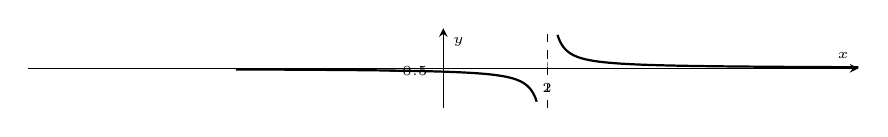
\begin{tikzpicture}[baseline=(current bounding box.north)]
\begin{axis}[
    width=\linewidth,
    height=2.6cm,
    axis lines=middle,
    xmin=-8, xmax=8,
    ymin=-6, ymax=6,
    xtick={2},
    ytick={-0.5},
    xticklabel style={font=\tiny},
    yticklabel style={font=\tiny},
    label style={font=\tiny},
    enlargelimits=false,
    samples=200,
    clip=false,
    xlabel={$x$},
    ylabel={$y$},
]
\addplot[thick, domain=-4:1.8] {1/(x-2)};
\addplot[thick, domain=2.2:8] {1/(x-2)};
\addplot[dashed] coordinates {(2,-6) (2,6)};
\end{axis}
\end{tikzpicture}
\\
\hline

1. Intercept(s)\par
a) x-int.\par
b) y-int.
&
a) $x=-3$\par
b) $y=9$
&
a) $x=0,-3$\par
b) $y=0$
&
a) $x=0,-3$\par
b) $y=0$
&
a) none\par
b) $y=-\dfrac12$
\\
\hline

2. End behaviour
&
$x\to\infty:\ +\infty$\par
$x\to-\infty:\ +\infty$
&
$x\to\infty:\ +\infty$\par
$x\to-\infty:\ -\infty$
&
$x\to\infty:\ +\infty$\par
$x\to-\infty:\ +\infty$
&
$x\to\infty:\ 0$\par
$x\to-\infty:\ 0$
\\
\hline

3. Critical points
&
$f'(x)=2(x+3)$\par
stat: $x=-3$
&
$f'(x)=3(x+3)(x+1)$\par
stat: $x=-3,-1$
&
$f'(x)=2x(x+3)(2x+3)$\par
stat: $x=-3,-\dfrac32,0$
&
$f'(x)=-\dfrac{1}{(x-2)^2}$\par
not diff. at $x=2$
\\
\hline

4. Dec./Inc.
&
dec: $(-\infty,-3)$\par
inc: $(-3,\infty)$
&
dec: $(-3,-1)$\par
inc: $(-\infty,-3)\cup(-1,\infty)$
&
dec: $(-\infty,-3)\cup\left(-\dfrac32,0\right)$\par
inc: $(-3,-\dfrac32)\cup(0,\infty)$
&
dec: $(-\infty,2)\cup(2,\infty)$\par
inc: none
\\
\hline

5. Rel. extremum
&
min: $(-3,0)$
&
max: $(-3,0)$\par
min: $(-1,-4)$
&
mins: $(-3,0),(0,0)$\par
max: $\left(-\dfrac32,\dfrac{81}{16}\right)$
&
none
\\
\hline

6. Concavity
&
up for all $x$
&
down: $(-\infty,-2)$\par
up: $(-2,\infty)$
&
up outside roots\par
down between roots
&
down: $(-\infty,2)$\par
up: $(2,\infty)$
\\
\hline

7. Inflection pt(s)
&
none
&
$(-2,-2)$
&
$\left(\dfrac{-3\pm\sqrt3}{2},\dfrac94\right)$
&
none
\\
\hline

8. Vert. asymp.
&
none
&
none
&
none
&
$x=2$
\\
\hline

9. Horiz. asymp.
&
none
&
none
&
none
&
$y=0$
\\
\hline

\end{tabularx}